%&preformat-present

\newif\ifpresentation % Условие, проверяющее, что документ --- презентация
\presentationtrue
\documentclass[10pt, xcolor={dvipsnames, table, hyperref}]{beamer}

%%%%%%%%%%%%%%%%%%%%%%%%%%%%%%%%%%%%%%%%%%%%%%%%%%%%%%%
%%%% Файл упрощённых настроек шаблона автореферата %%%%
%%%%%%%%%%%%%%%%%%%%%%%%%%%%%%%%%%%%%%%%%%%%%%%%%%%%%%%

%%% Инициализирование переменных, не трогать!  %%%
\newcounter{showperssign}
\newcounter{showsecrsign}
\newcounter{showopplead}
%%%%%%%%%%%%%%%%%%%%%%%%%%%%%%%%%%%%%%%%%%%%%%%%%%%%%%%

%%% Список публикаций %%%
\makeatletter
\@ifundefined{c@usefootcite}{
  \newcounter{usefootcite}
  \setcounter{usefootcite}{0} % 0 --- два списка литературы;
                              % 1 --- список публикаций автора + цитирование
                              %       других работ в сносках
}{}
\makeatother

\makeatletter
\@ifundefined{c@bibgrouped}{
  \newcounter{bibgrouped}
  \setcounter{bibgrouped}{0}  % 0 --- единый список работ автора;
                              % 1 --- сгруппированные работы автора
}{}
\makeatother

%%% Область упрощённого управления оформлением %%%

%% Управление зазором между подрисуночной подписью и основным текстом %%
\setlength{\belowcaptionskip}{10pt plus 20pt minus 2pt}


%% Подпись таблиц %%

% смещение строк подписи после первой
\newcommand{\tabindent}{0cm}

% тип форматирования таблицы
% plain --- название и текст в одной строке
% split --- название и текст в разных строках
\newcommand{\tabformat}{plain}

%%% настройки форматирования таблицы `plain'

% выравнивание по центру подписи, состоящей из одной строки
% true  --- выравнивать
% false --- не выравнивать
\newcommand{\tabsinglecenter}{false}

% выравнивание подписи таблиц
% justified   --- выравнивать как обычный текст
% centering   --- выравнивать по центру
% centerlast  --- выравнивать по центру только последнюю строку
% centerfirst --- выравнивать по центру только первую строку
% raggedleft  --- выравнивать по правому краю
% raggedright --- выравнивать по левому краю
\newcommand{\tabjust}{justified}

% Разделитель записи «Таблица #» и названия таблицы
\newcommand{\tablabelsep}{~\cyrdash\ }

%%% настройки форматирования таблицы `split'

% положение названия таблицы
% \centering   --- выравнивать по центру
% \raggedleft  --- выравнивать по правому краю
% \raggedright --- выравнивать по левому краю
\newcommand{\splitformatlabel}{\raggedleft}

% положение текста подписи
% \centering   --- выравнивать по центру
% \raggedleft  --- выравнивать по правому краю
% \raggedright --- выравнивать по левому краю
\newcommand{\splitformattext}{\raggedright}

%% Подпись рисунков %%
%Разделитель записи «Рисунок #» и названия рисунка
\newcommand{\figlabelsep}{~\cyrdash\ }  % (ГОСТ 2.105, 4.3.1)
                                        % "--- здесь не работает

%Демонстрация подписи диссертанта на автореферате
\setcounter{showperssign}{1}  % 0 --- не показывать;
                              % 1 --- показывать
%Демонстрация подписи учёного секретаря на автореферате
\setcounter{showsecrsign}{1}  % 0 --- не показывать;
                              % 1 --- показывать
%Демонстрация информации об оппонентах и ведущей организации на автореферате
\setcounter{showopplead}{1}   % 0 --- не показывать;
                              % 1 --- показывать

%%% Цвета гиперссылок %%%
% Latex color definitions: http://latexcolor.com/
\definecolor{linkcolor}{rgb}{0.9,0,0}
\definecolor{citecolor}{rgb}{0,0.6,0}
\definecolor{urlcolor}{rgb}{0,0,1}
%\definecolor{linkcolor}{rgb}{0,0,0} %black
%\definecolor{citecolor}{rgb}{0,0,0} %black
%\definecolor{urlcolor}{rgb}{0,0,0} %black
               % Общие настройки шаблона
\input{common/packages}            % Пакеты общие для диссертации и автореферата
%%% Основные сведения %%%
\newcommand{\thesisAuthorLastName}{Подкурков}
\newcommand{\thesisAuthorOtherNames}{Иван Алексеевич}
\newcommand{\thesisAuthorInitials}{И.\,А.}
\newcommand{\thesisAuthor}             % Диссертация, ФИО автора
{%
    \texorpdfstring{% \texorpdfstring takes two arguments and uses the first for (La)TeX and the second for pdf
        \thesisAuthorLastName~\thesisAuthorOtherNames% так будет отображаться на титульном листе или в тексте, где будет использоваться переменная
    }{%
        \thesisAuthorLastName, \thesisAuthorOtherNames% эта запись для свойств pdf-файла. В таком виде, если pdf будет обработан программами для сбора библиографических сведений, будет правильно представлена фамилия.
    }
}
\newcommand{\thesisAuthorShort}        % Диссертация, ФИО автора инициалами
{\thesisAuthorInitials~\thesisAuthorLastName}
%\newcommand{\thesisUdk}                % Диссертация, УДК
%{\fixme{xxx.xxx}}
\newcommand{\thesisTitle}              % Диссертация, название
{Разработка и анализ потенциальных характеристик алгоритмов оценивания параметров многомерных сигналов в инфокоммуникационных системах}
\newcommand{\thesisSpecialtyNumber}    % Диссертация, специальность, номер
{05.12.13}
\newcommand{\thesisSpecialtyTitle}     % Диссертация, специальность, название (название взято с сайта ВАК для примера)
{Системы, сети и устройства телекоммуникаций}
%% \newcommand{\thesisSpecialtyTwoNumber} % Диссертация, вторая специальность, номер
%% {\fixme{XX.XX.XX}}
%% \newcommand{\thesisSpecialtyTwoTitle}  % Диссертация, вторая специальность, название
%% {\fixme{Теория и~методика физического воспитания, спортивной тренировки,
%% оздоровительной и~адаптивной физической культуры}}
\newcommand{\thesisDegree}             % Диссертация, ученая степень
{кандидата технических наук}
\newcommand{\thesisDegreeShort}        % Диссертация, ученая степень, краткая запись
{канд. техн. наук}
\newcommand{\thesisCity}               % Диссертация, город написания диссертации
{Казань}
\newcommand{\thesisYear}               % Диссертация, год написания диссертации
{2020}
\newcommand{\thesisOrganization}       % Диссертация, организация
{Федеральное государственное автономное образовательное учреждение высшего
образования <<Казанский Национальный Исследовательский Технический Университет им. А. Н. Туполева <<КНИТУ-КАИ>>}
\newcommand{\thesisOrganizationShort}  % Диссертация, краткое название организации для доклада
{\fixme{КНИТУ-КАИ}}

\newcommand{\thesisInOrganization}     % Диссертация, организация в предложном падеже: Работа выполнена в ...
{Казанском Национальном Исследовательском Техническом Университете им. А. Н. Туполева}

%% \newcommand{\supervisorDead}{}           % Рисовать рамку вокруг фамилии
\newcommand{\supervisorFio}              % Научный руководитель, ФИО
{Надеев Адель Фирадович}
\newcommand{\supervisorRegalia}          % Научный руководитель, регалии
{доктор физико-математических наук, профессор}
\newcommand{\supervisorFioShort}         % Научный руководитель, ФИО
{А.\,Ф.~Надеев}
\newcommand{\supervisorRegaliaShort}     % Научный руководитель, регалии
{д.~ф.~-~м.~н.,~проф.}

%% \newcommand{\supervisorTwoDead}{}        % Рисовать рамку вокруг фамилии
%% \newcommand{\supervisorTwoFio}           % Второй научный руководитель, ФИО
%% {\fixme{Фамилия Имя Отчество}}
%% \newcommand{\supervisorTwoRegalia}       % Второй научный руководитель, регалии
%% {\fixme{уч. степень, уч. звание}}
%% \newcommand{\supervisorTwoFioShort}      % Второй научный руководитель, ФИО
%% {\fixme{И.\,О.~Фамилия}}
%% \newcommand{\supervisorTwoRegaliaShort}  % Второй научный руководитель, регалии
%% {\fixme{уч.~ст.,~уч.~зв.}}

\newcommand{\opponentOneFio}           % Оппонент 1, ФИО
{\fixme{Фамилия Имя Отчество}}
\newcommand{\opponentOneRegalia}       % Оппонент 1, регалии
{\fixme{доктор физико-математических наук, профессор}}
\newcommand{\opponentOneJobPlace}      % Оппонент 1, место работы
{\fixme{Не очень длинное название для места работы}}
\newcommand{\opponentOneJobPost}       % Оппонент 1, должность
{\fixme{старший научный сотрудник}}

\newcommand{\opponentTwoFio}           % Оппонент 2, ФИО
{\fixme{Фамилия Имя Отчество}}
\newcommand{\opponentTwoRegalia}       % Оппонент 2, регалии
{\fixme{кандидат физико-математических наук}}
\newcommand{\opponentTwoJobPlace}      % Оппонент 2, место работы
{\fixme{Основное место работы c длинным длинным длинным длинным названием}}
\newcommand{\opponentTwoJobPost}       % Оппонент 2, должность
{\fixme{старший научный сотрудник}}

%% \newcommand{\opponentThreeFio}         % Оппонент 3, ФИО
%% {\fixme{Фамилия Имя Отчество}}
%% \newcommand{\opponentThreeRegalia}     % Оппонент 3, регалии
%% {\fixme{кандидат физико-математических наук}}
%% \newcommand{\opponentThreeJobPlace}    % Оппонент 3, место работы
%% {\fixme{Основное место работы c длинным длинным длинным длинным названием}}
%% \newcommand{\opponentThreeJobPost}     % Оппонент 3, должность
%% {\fixme{старший научный сотрудник}}

\newcommand{\leadingOrganizationTitle} % Ведущая организация, дополнительные строки. Удалить, чтобы не отображать в автореферате
{\fixme{Федеральное государственное бюджетное образовательное учреждение высшего
профессионального образования с~длинным длинным длинным длинным названием}}

\newcommand{\defenseDate}              % Защита, дата
{\fixme{DD mmmmmmmm YYYY~г.~в~XX часов}}
\newcommand{\defenseCouncilNumber}     % Защита, номер диссертационного совета
{\fixme{Д\,123.456.78}}
\newcommand{\defenseCouncilTitle}      % Защита, учреждение диссертационного совета
{\fixme{Название учреждения}}
\newcommand{\defenseCouncilAddress}    % Защита, адрес учреждение диссертационного совета
{\fixme{Адрес}}
\newcommand{\defenseCouncilPhone}      % Телефон для справок
{\fixme{+7~(0000)~00-00-00}}

\newcommand{\defenseSecretaryFio}      % Секретарь диссертационного совета, ФИО
{\fixme{Фамилия Имя Отчество}}
\newcommand{\defenseSecretaryRegalia}  % Секретарь диссертационного совета, регалии
{\fixme{д-р~физ.-мат. наук}}            % Для сокращений есть ГОСТы, например: ГОСТ Р 7.0.12-2011 + http://base.garant.ru/179724/#block_30000

\newcommand{\synopsisLibrary}          % Автореферат, название библиотеки
{\fixme{Название библиотеки}}
\newcommand{\synopsisDate}             % Автореферат, дата рассылки
{\fixme{DD mmmmmmmm YYYY года}}

% To avoid conflict with beamer class use \providecommand
\providecommand{\keywords}%            % Ключевые слова для метаданных PDF диссертации и автореферата
{}
                % Основные сведения
\input{common/fonts}               % Определение шрифтов (частичное)

%%%%%%%%%%%%%%%%%%%%%%%%%%%%%%%%%%%%%%%%%%%%%%%%%%%%%%%
%%%% Файл упрощённых настроек шаблона автореферата %%%%
%%%%%%%%%%%%%%%%%%%%%%%%%%%%%%%%%%%%%%%%%%%%%%%%%%%%%%%

%%% Инициализирование переменных, не трогать!  %%%
\newcounter{showperssign}
\newcounter{showsecrsign}
\newcounter{showopplead}
%%%%%%%%%%%%%%%%%%%%%%%%%%%%%%%%%%%%%%%%%%%%%%%%%%%%%%%

%%% Список публикаций %%%
\makeatletter
\@ifundefined{c@usefootcite}{
  \newcounter{usefootcite}
  \setcounter{usefootcite}{0} % 0 --- два списка литературы;
                              % 1 --- список публикаций автора + цитирование
                              %       других работ в сносках
}{}
\makeatother

\makeatletter
\@ifundefined{c@bibgrouped}{
  \newcounter{bibgrouped}
  \setcounter{bibgrouped}{0}  % 0 --- единый список работ автора;
                              % 1 --- сгруппированные работы автора
}{}
\makeatother

%%% Область упрощённого управления оформлением %%%

%% Управление зазором между подрисуночной подписью и основным текстом %%
\setlength{\belowcaptionskip}{10pt plus 20pt minus 2pt}


%% Подпись таблиц %%

% смещение строк подписи после первой
\newcommand{\tabindent}{0cm}

% тип форматирования таблицы
% plain --- название и текст в одной строке
% split --- название и текст в разных строках
\newcommand{\tabformat}{plain}

%%% настройки форматирования таблицы `plain'

% выравнивание по центру подписи, состоящей из одной строки
% true  --- выравнивать
% false --- не выравнивать
\newcommand{\tabsinglecenter}{false}

% выравнивание подписи таблиц
% justified   --- выравнивать как обычный текст
% centering   --- выравнивать по центру
% centerlast  --- выравнивать по центру только последнюю строку
% centerfirst --- выравнивать по центру только первую строку
% raggedleft  --- выравнивать по правому краю
% raggedright --- выравнивать по левому краю
\newcommand{\tabjust}{justified}

% Разделитель записи «Таблица #» и названия таблицы
\newcommand{\tablabelsep}{~\cyrdash\ }

%%% настройки форматирования таблицы `split'

% положение названия таблицы
% \centering   --- выравнивать по центру
% \raggedleft  --- выравнивать по правому краю
% \raggedright --- выравнивать по левому краю
\newcommand{\splitformatlabel}{\raggedleft}

% положение текста подписи
% \centering   --- выравнивать по центру
% \raggedleft  --- выравнивать по правому краю
% \raggedright --- выравнивать по левому краю
\newcommand{\splitformattext}{\raggedright}

%% Подпись рисунков %%
%Разделитель записи «Рисунок #» и названия рисунка
\newcommand{\figlabelsep}{~\cyrdash\ }  % (ГОСТ 2.105, 4.3.1)
                                        % "--- здесь не работает

%Демонстрация подписи диссертанта на автореферате
\setcounter{showperssign}{1}  % 0 --- не показывать;
                              % 1 --- показывать
%Демонстрация подписи учёного секретаря на автореферате
\setcounter{showsecrsign}{1}  % 0 --- не показывать;
                              % 1 --- показывать
%Демонстрация информации об оппонентах и ведущей организации на автореферате
\setcounter{showopplead}{1}   % 0 --- не показывать;
                              % 1 --- показывать

%%% Цвета гиперссылок %%%
% Latex color definitions: http://latexcolor.com/
\definecolor{linkcolor}{rgb}{0.9,0,0}
\definecolor{citecolor}{rgb}{0,0.6,0}
\definecolor{urlcolor}{rgb}{0,0,1}
%\definecolor{linkcolor}{rgb}{0,0,0} %black
%\definecolor{citecolor}{rgb}{0,0,0} %black
%\definecolor{urlcolor}{rgb}{0,0,0} %black
         % Настройки презентации
\input{Presentation/prespackages}  % Библиотеки презентации
% Общие стили оформления.
% Возможные варианты значений ищите в описании библиотеки beamer
\usetheme{Pittsburgh}
\usecolortheme{whale}

% \usetheme[secheader]{Boadilla}
% \usecolortheme{seahorse}

% выключение кнопок навигации
\beamertemplatenavigationsymbolsempty

% Размеры шрифтов
\setbeamerfont{title}{size=\large}
\setbeamerfont{subtitle}{size=\small}
\setbeamerfont{author}{size=\normalsize}
\setbeamerfont{institute}{size=\small}
\setbeamerfont{date}{size=\normalsize}
\setbeamerfont{bibliography item}{size=\small}
\setbeamerfont{bibliography entry author}{size=\small}
\setbeamerfont{bibliography entry title}{size=\small}
\setbeamerfont{bibliography entry location}{size=\small}
\setbeamerfont{bibliography entry note}{size=\small}
% Аналогично можно настроить и другие размеры.
% Названия классов элементов можно найти здесь
% http://www.cpt.univ-mrs.fr/~masson/latex/Beamer-appearance-cheat-sheet.pdf

% Цвет элементов
\setbeamercolor{footline}{fg=blue}
\setbeamercolor{bibliography item}{fg=black}
\setbeamercolor{bibliography entry author}{fg=black}
\setbeamercolor{bibliography entry title}{fg=black}
\setbeamercolor{bibliography entry location}{fg=black}
\setbeamercolor{bibliography entry note}{fg=black}
% Аналогично можно настроить и другие цвета.
% Названия классов элементов можно найти здесь
% http://www.cpt.univ-mrs.fr/~masson/latex/Beamer-appearance-cheat-sheet.pdf

% Убрать иконки перед списком литературы
% https://tex.stackexchange.com/a/124271/104425
%\setbeamertemplate{bibliography item}{}
\setbeamertemplate{bibliography item}{\insertbiblabel}

% Использовать шрифт с засечками для формул
% https://tex.stackexchange.com/a/34267/104425
\usefonttheme[onlymath]{serif}

% https://tex.stackexchange.com/a/291545/104425
\makeatletter
\def\beamer@framenotesbegin{% at beginning of slide
    \usebeamercolor[fg]{normal text}
    \gdef\beamer@noteitems{}%
    \gdef\beamer@notes{}%
}
\makeatother

% footer презентации
\setbeamertemplate{footline}{
    \leavevmode%
    \hbox{%
        \begin{beamercolorbox}[wd=.333333\paperwidth,ht=2.25ex,dp=1ex,center]{}%
            % И. О. Фамилия, Организация кратко
            \thesisAuthorShort, \thesisOrganizationShort
        \end{beamercolorbox}%
        \begin{beamercolorbox}[wd=.333333\paperwidth,ht=2.25ex,dp=1ex,center]{}%
            % Город, 20XX
            \thesisCity, \thesisYear
        \end{beamercolorbox}%
        \begin{beamercolorbox}[wd=.333333\paperwidth,ht=2.25ex,dp=1ex,right]{}%
            Стр. \insertframenumber{} из \inserttotalframenumber \hspace*{2ex}
        \end{beamercolorbox}}%
    \vskip0pt%
}

% вывод на экран заметок к презентации
\ifnumequal{\value{presnotes}}{0}{}{
    \setbeameroption{show notes}
    \ifnumequal{\value{presnotes}}{2}{
        \setbeameroption{show notes on second screen=\presposition}
    }{}
}
        % Стили презентации
\setbeamertemplate{title page}
{
    \ifnumequal{\value{logotitle}}{1}{
        \IfFileExists{images/logo-knitu.pdf}{
            \begin{minipage}[c]{0.15\textwidth}
                \begin{flushleft}
                    \usebeamercolor[fg]{titlegraphic}\inserttitlegraphic
                \end{flushleft}
            \end{minipage}%
            \hfill
            \begin{minipage}[c]{0.8\linewidth}
                \centering
                \usebeamerfont{institute}\insertinstitute\par
            \end{minipage}
        }{
            \centering
            \usebeamerfont{institute}\insertinstitute\par
        }
    }{
        \centering
        \usebeamerfont{institute}\insertinstitute\par
    }
    \centering
    \vfill
    \usebeamerfont{subtitle}\insertsubtitle\par
    \bigskip
    \usebeamerfont{title}\inserttitle\par
    \vfill
    \usebeamerfont{author}\insertauthor\par
    \vfill
    \usebeamerfont{date}\insertdate\par
}

%\title{\small{Название презентации}}
\title{\thesisTitle}
\author{%
    \texorpdfstring{%
        \emph{Выступающий:}~\thesisAuthorShort\\%
        \emph{Руководители:}~\supervisorRegaliaShort~\supervisorFioShort\\%
        \emph{\ \ \ \ \ \ \ \ \ \ \ \ \ \ \ \ \ \ \ }~Univ.-Prof.~Dr.-Ing.~Martin~Haardt\\%
        %
    }{\thesisAuthor}%
}
\date{\texorpdfstring{\thesisCity, \thesisYear}{}}
\institute{\texorpdfstring{\thesisOrganization}{}}
\IfFileExists{images/logo-knitu.pdf}{
    \titlegraphic{
\includegraphics[width=\textwidth]{images/logo-knitu}}
    \ifnumequal{\value{logoother}}{1}{
        \logo{
\includegraphics[width=0.15\textwidth]{images/logo-knitu}}
    }{}
}{}
\subtitle{Представление научного доклада по специальности \\ \thesisSpecialtyNumber\ \thesisSpecialtyTitle}
         % Настройки заглавной странице
% для вертикального центрирования ячеек в tabulary
\def\zz{\ifx\[$\else\aftergroup\zzz\fi}
%$ \] % <-- чиним подсветку синтаксиса в некоторых редакторах
\def\zzz{\setbox0\lastbox
\dimen0\dimexpr\extrarowheight + \ht0-\dp0\relax
\setbox0\hbox{\raise-.5\dimen0\box0}%
\ht0=\dimexpr\ht0+\extrarowheight\relax
\dp0=\dimexpr\dp0+\extrarowheight\relax
\box0
}

\lstdefinelanguage{Renhanced}%
{keywords={abbreviate,abline,abs,acos,acosh,action,add1,add,%
        aggregate,alias,Alias,alist,all,anova,any,aov,aperm,append,apply,%
        approx,approxfun,apropos,Arg,args,array,arrows,as,asin,asinh,%
        atan,atan2,atanh,attach,attr,attributes,autoload,autoloader,ave,%
        axis,backsolve,barplot,basename,besselI,besselJ,besselK,besselY,%
        beta,binomial,body,box,boxplot,break,browser,bug,builtins,bxp,by,%
        c,C,call,Call,case,cat,category,cbind,ceiling,character,char,%
        charmatch,check,chol,chol2inv,choose,chull,class,close,cm,codes,%
        coef,coefficients,co,col,colnames,colors,colours,commandArgs,%
        comment,complete,complex,conflicts,Conj,contents,contour,%
        contrasts,contr,control,helmert,contrib,convolve,cooks,coords,%
        distance,coplot,cor,cos,cosh,count,fields,cov,covratio,wt,CRAN,%
        create,crossprod,cummax,cummin,cumprod,cumsum,curve,cut,cycle,D,%
        data,dataentry,date,dbeta,dbinom,dcauchy,dchisq,de,debug,%
        debugger,Defunct,default,delay,delete,deltat,demo,de,density,%
        deparse,dependencies,Deprecated,deriv,description,detach,%
        dev2bitmap,dev,cur,deviance,off,prev,,dexp,df,dfbetas,dffits,%
        dgamma,dgeom,dget,dhyper,diag,diff,digamma,dim,dimnames,dir,%
        dirname,dlnorm,dlogis,dnbinom,dnchisq,dnorm,do,dotplot,double,%
        download,dpois,dput,drop,drop1,dsignrank,dt,dummy,dump,dunif,%
        duplicated,dweibull,dwilcox,dyn,edit,eff,effects,eigen,else,%
        emacs,end,environment,env,erase,eval,equal,evalq,example,exists,%
        exit,exp,expand,expression,External,extract,extractAIC,factor,%
        fail,family,fft,file,filled,find,fitted,fivenum,fix,floor,for,%
        For,formals,format,formatC,formula,Fortran,forwardsolve,frame,%
        frequency,ftable,ftable2table,function,gamma,Gamma,gammaCody,%
        gaussian,gc,gcinfo,gctorture,get,getenv,geterrmessage,getOption,%
        getwd,gl,glm,globalenv,gnome,GNOME,graphics,gray,grep,grey,grid,%
        gsub,hasTsp,hat,heat,help,hist,home,hsv,httpclient,I,identify,if,%
        ifelse,Im,image,\%in\%,index,influence,measures,inherits,install,%
        installed,integer,interaction,interactive,Internal,intersect,%
        inverse,invisible,IQR,is,jitter,kappa,kronecker,labels,lapply,%
        layout,lbeta,lchoose,lcm,legend,length,levels,lgamma,library,%
        licence,license,lines,list,lm,load,local,locator,log,log10,log1p,%
        log2,logical,loglin,lower,lowess,ls,lsfit,lsf,ls,machine,Machine,%
        mad,mahalanobis,make,link,margin,match,Math,matlines,mat,matplot,%
        matpoints,matrix,max,mean,median,memory,menu,merge,methods,min,%
        missing,Mod,mode,model,response,mosaicplot,mtext,mvfft,na,nan,%
        names,omit,nargs,nchar,ncol,NCOL,new,next,NextMethod,nextn,%
        nlevels,nlm,noquote,NotYetImplemented,NotYetUsed,nrow,NROW,null,%
        numeric,\%o\%,objects,offset,old,on,Ops,optim,optimise,optimize,%
        options,or,order,ordered,outer,package,packages,page,pairlist,%
        pairs,palette,panel,par,parent,parse,paste,path,pbeta,pbinom,%
        pcauchy,pchisq,pentagamma,persp,pexp,pf,pgamma,pgeom,phyper,pico,%
        pictex,piechart,Platform,plnorm,plogis,plot,pmatch,pmax,pmin,%
        pnbinom,pnchisq,pnorm,points,poisson,poly,polygon,polyroot,pos,%
        postscript,power,ppoints,ppois,predict,preplot,pretty,Primitive,%
        print,prmatrix,proc,prod,profile,proj,prompt,prop,provide,%
        psignrank,ps,pt,ptukey,punif,pweibull,pwilcox,q,qbeta,qbinom,%
        qcauchy,qchisq,qexp,qf,qgamma,qgeom,qhyper,qlnorm,qlogis,qnbinom,%
        qnchisq,qnorm,qpois,qqline,qqnorm,qqplot,qr,Q,qty,qy,qsignrank,%
        qt,qtukey,quantile,quasi,quit,qunif,quote,qweibull,qwilcox,%
        rainbow,range,rank,rbeta,rbind,rbinom,rcauchy,rchisq,Re,read,csv,%
        csv2,fwf,readline,socket,real,Recall,rect,reformulate,regexpr,%
        relevel,remove,rep,repeat,replace,replications,report,require,%
        resid,residuals,restart,return,rev,rexp,rf,rgamma,rgb,rgeom,R,%
        rhyper,rle,rlnorm,rlogis,rm,rnbinom,RNGkind,rnorm,round,row,%
        rownames,rowsum,rpois,rsignrank,rstandard,rstudent,rt,rug,runif,%
        rweibull,rwilcox,sample,sapply,save,scale,scan,scan,screen,sd,se,%
        search,searchpaths,segments,seq,sequence,setdiff,setequal,set,%
        setwd,show,sign,signif,sin,single,sinh,sink,solve,sort,source,%
        spline,splinefun,split,sqrt,stars,start,stat,stem,step,stop,%
        storage,strstrheight,stripplot,strsplit,structure,strwidth,sub,%
        subset,substitute,substr,substring,sum,summary,sunflowerplot,svd,%
        sweep,switch,symbol,symbols,symnum,sys,status,system,t,table,%
        tabulate,tan,tanh,tapply,tempfile,terms,terrain,tetragamma,text,%
        time,title,topo,trace,traceback,transform,tri,trigamma,trunc,try,%
        ts,tsp,typeof,unclass,undebug,undoc,union,unique,uniroot,unix,%
        unlink,unlist,unname,untrace,update,upper,url,UseMethod,var,%
        variable,vector,Version,vi,warning,warnings,weighted,weights,%
        which,while,window,write,\%x\%,x11,X11,xedit,xemacs,xinch,xor,%
        xpdrows,xy,xyinch,yinch,zapsmall,zip},%
    otherkeywords={!,!=,~,$,*,\%,\&,\%/\%,\%*\%,\%\%,<-,<<-},%$
    alsoother={._$},%$
    sensitive,%
    morecomment=[l]\#,%
    morestring=[d]",%
    morestring=[d]'% 2001 Robert Denham
}%

%решаем проблему с кириллицей в комментариях (в pdflatex) https://tex.stackexchange.com/a/103712
\lstset{extendedchars=true,keepspaces=true,literate={Ö}{{\"O}}1
    {Ä}{{\"A}}1
    {Ü}{{\"U}}1
    {ß}{{\ss}}1
    {ü}{{\"u}}1
    {ä}{{\"a}}1
    {ö}{{\"o}}1
    {~}{{\textasciitilde}}1
    {а}{{\selectfont\char224}}1
    {б}{{\selectfont\char225}}1
    {в}{{\selectfont\char226}}1
    {г}{{\selectfont\char227}}1
    {д}{{\selectfont\char228}}1
    {е}{{\selectfont\char229}}1
    {ё}{{\"e}}1
    {ж}{{\selectfont\char230}}1
    {з}{{\selectfont\char231}}1
    {и}{{\selectfont\char232}}1
    {й}{{\selectfont\char233}}1
    {к}{{\selectfont\char234}}1
    {л}{{\selectfont\char235}}1
    {м}{{\selectfont\char236}}1
    {н}{{\selectfont\char237}}1
    {о}{{\selectfont\char238}}1
    {п}{{\selectfont\char239}}1
    {р}{{\selectfont\char240}}1
    {с}{{\selectfont\char241}}1
    {т}{{\selectfont\char242}}1
    {у}{{\selectfont\char243}}1
    {ф}{{\selectfont\char244}}1
    {х}{{\selectfont\char245}}1
    {ц}{{\selectfont\char246}}1
    {ч}{{\selectfont\char247}}1
    {ш}{{\selectfont\char248}}1
    {щ}{{\selectfont\char249}}1
    {ъ}{{\selectfont\char250}}1
    {ы}{{\selectfont\char251}}1
    {ь}{{\selectfont\char252}}1
    {э}{{\selectfont\char253}}1
    {ю}{{\selectfont\char254}}1
    {я}{{\selectfont\char255}}1
    {А}{{\selectfont\char192}}1
    {Б}{{\selectfont\char193}}1
    {В}{{\selectfont\char194}}1
    {Г}{{\selectfont\char195}}1
    {Д}{{\selectfont\char196}}1
    {Е}{{\selectfont\char197}}1
    {Ё}{{\"E}}1
    {Ж}{{\selectfont\char198}}1
    {З}{{\selectfont\char199}}1
    {И}{{\selectfont\char200}}1
    {Й}{{\selectfont\char201}}1
    {К}{{\selectfont\char202}}1
    {Л}{{\selectfont\char203}}1
    {М}{{\selectfont\char204}}1
    {Н}{{\selectfont\char205}}1
    {О}{{\selectfont\char206}}1
    {П}{{\selectfont\char207}}1
    {Р}{{\selectfont\char208}}1
    {С}{{\selectfont\char209}}1
    {Т}{{\selectfont\char210}}1
    {У}{{\selectfont\char211}}1
    {Ф}{{\selectfont\char212}}1
    {Х}{{\selectfont\char213}}1
    {Ц}{{\selectfont\char214}}1
    {Ч}{{\selectfont\char215}}1
    {Ш}{{\selectfont\char216}}1
    {Щ}{{\selectfont\char217}}1
    {Ъ}{{\selectfont\char218}}1
    {Ы}{{\selectfont\char219}}1
    {Ь}{{\selectfont\char220}}1
    {Э}{{\selectfont\char221}}1
    {Ю}{{\selectfont\char222}}1
    {Я}{{\selectfont\char223}}1
    {і}{{\selectfont\char105}}1
    {ї}{{\selectfont\char168}}1
    {є}{{\selectfont\char185}}1
    {ґ}{{\selectfont\char160}}1
    {І}{{\selectfont\char73}}1
    {Ї}{{\selectfont\char136}}1
    {Є}{{\selectfont\char153}}1
    {Ґ}{{\selectfont\char128}}1
}

% Ширина текста минус ширина надписи 999
\newlength{\twless}
\newlength{\lmarg}
\setlength{\lmarg}{\widthof{999}}   % ширина надписи 999
\setlength{\twless}{\textwidth-\lmarg}

\lstset{ %
%    language=R,                     %  Язык указать здесь, если во всех листингах преимущественно один язык, в результате часть настроек может пойти только для этого языка
    numbers=left,                   % where to put the line-numbers
    numberstyle=\fontsize{12pt}{14pt}\selectfont\color{Gray},  % the style that is used for the line-numbers
    firstnumber=1,                  % в этой и следующей строках задаётся поведение нумерации 5, 10, 15...
    stepnumber=5,                   % the step between two line-numbers. If it's 1, each line will be numbered
    numbersep=5pt,                  % how far the line-numbers are from the code
    backgroundcolor=\color{white},  % choose the background color. You must add \usepackage{color}
    showspaces=false,               % show spaces adding particular underscores
    showstringspaces=false,         % underline spaces within strings
    showtabs=false,                 % show tabs within strings adding particular underscores
    frame=leftline,                 % adds a frame of different types around the code
    rulecolor=\color{black},        % if not set, the frame-color may be changed on line-breaks within not-black text (e.g. commens (green here))
    tabsize=2,                      % sets default tabsize to 2 spaces
    captionpos=t,                   % sets the caption-position to top
    breaklines=true,                % sets automatic line breaking
    breakatwhitespace=false,        % sets if automatic breaks should only happen at whitespace
%    title=\lstname,                 % show the filename of files included with \lstinputlisting;
    % also try caption instead of title
    basicstyle=\fontsize{12pt}{14pt}\selectfont\ttfamily,% the size of the fonts that are used for the code
%    keywordstyle=\color{blue},      % keyword style
    commentstyle=\color{ForestGreen}\emph,% comment style
    stringstyle=\color{Mahogany},   % string literal style
    escapeinside={\%*}{*)},         % if you want to add a comment within your code
    morekeywords={*,...},           % if you want to add more keywords to the set
    inputencoding=utf8,             % кодировка кода
    xleftmargin={\lmarg},           % Чтобы весь код и полоска с номерами строк была смещена влево, так чтобы цифры не вылезали за пределы текста слева
}

%http://tex.stackexchange.com/questions/26872/smaller-frame-with-listings
% Окружение, чтобы листинг был компактнее обведен рамкой, если она задается, а не на всю ширину текста
\makeatletter
\newenvironment{SmallListing}[1][]
{\lstset{#1}\VerbatimEnvironment\begin{VerbatimOut}{VerbEnv.tmp}}
{\end{VerbatimOut}\settowidth\@tempdima{%
        \lstinputlisting{VerbEnv.tmp}}
    \minipage{\@tempdima}\lstinputlisting{VerbEnv.tmp}\endminipage}
\makeatother

\DefineVerbatimEnvironment% с шрифтом 12 пт
{Verb}{Verbatim}
{fontsize=\fontsize{12pt}{14pt}\selectfont}

\newfloat[chapter]{ListingEnv}{lol}{Листинг}

\renewcommand{\lstlistingname}{Листинг}

%Общие счётчики окружений листингов
%http://tex.stackexchange.com/questions/145546/how-to-make-figure-and-listing-share-their-counter
% Если смешивать плавающие и не плавающие окружения, то могут быть проблемы с нумерацией
\makeatletter
\AtBeginDocument{%
    \let\c@ListingEnv\c@lstlisting
    \let\theListingEnv\thelstlisting
    \let\ftype@lstlisting\ftype@ListingEnv % give the floats the same precedence
}
\makeatother

% значок С++ — используйте команду \cpp
\newcommand{\cpp}{%
    C\nolinebreak\hspace{-.05em}%
    \raisebox{.2ex}{+}\nolinebreak\hspace{-.10em}%
    \raisebox{.2ex}{+}%
}

%%%  Чересстрочное форматирование таблиц
%% http://tex.stackexchange.com/questions/278362/apply-italic-formatting-to-every-other-row
\newcounter{rowcnt}
\newcommand\altshape{\ifnumodd{\value{rowcnt}}{\color{red}}{\vspace*{-1ex}\itshape}}
% \AtBeginEnvironment{tabular}{\setcounter{rowcnt}{1}}
% \AtEndEnvironment{tabular}{\setcounter{rowcnt}{0}}

%%% Ради примера во второй главе
\let\originalepsilon\epsilon
\let\originalphi\phi
\let\originalkappa\kappa
\let\originalle\le
\let\originalleq\leq
\let\originalge\ge
\let\originalgeq\geq
\let\originalemptyset\emptyset
\let\originaltan\tan
\let\originalcot\cot
\let\originalcsc\csc

%%% Русская традиция начертания математических знаков
\renewcommand{\le}{\ensuremath{\leqslant}}
\renewcommand{\leq}{\ensuremath{\leqslant}}
\renewcommand{\ge}{\ensuremath{\geqslant}}
\renewcommand{\geq}{\ensuremath{\geqslant}}
\renewcommand{\emptyset}{\varnothing}

%%% Русская традиция начертания математических функций (на случай копирования из зарубежных источников)
\renewcommand{\tan}{\operatorname{tg}}
\renewcommand{\cot}{\operatorname{ctg}}
\renewcommand{\csc}{\operatorname{cosec}}

%%% Русская традиция начертания греческих букв (греческие буквы вертикальные, через пакет upgreek)
\renewcommand{\epsilon}{\ensuremath{\upvarepsilon}}   %  русская традиция записи
\renewcommand{\phi}{\ensuremath{\upvarphi}}
%\renewcommand{\kappa}{\ensuremath{\varkappa}}
\renewcommand{\alpha}{\upalpha}
\renewcommand{\beta}{\upbeta}
\renewcommand{\gamma}{\upgamma}
\renewcommand{\delta}{\updelta}
\renewcommand{\varepsilon}{\upvarepsilon}
\renewcommand{\zeta}{\upzeta}
\renewcommand{\eta}{\upeta}
\renewcommand{\theta}{\uptheta}
\renewcommand{\vartheta}{\upvartheta}
\renewcommand{\iota}{\upiota}
\renewcommand{\kappa}{\upkappa}
\renewcommand{\lambda}{\uplambda}
\renewcommand{\mu}{\upmu}
\renewcommand{\nu}{\upnu}
\renewcommand{\xi}{\upxi}
\renewcommand{\pi}{\uppi}
\renewcommand{\varpi}{\upvarpi}
\renewcommand{\rho}{\uprho}
%\renewcommand{\varrho}{\upvarrho}
\renewcommand{\sigma}{\upsigma}
%\renewcommand{\varsigma}{\upvarsigma}
\renewcommand{\tau}{\uptau}
\renewcommand{\upsilon}{\upupsilon}
\renewcommand{\varphi}{\upvarphi}
\renewcommand{\chi}{\upchi}
\renewcommand{\psi}{\uppsi}
\renewcommand{\omega}{\upomega}
%%% Микротипографика %%%
%\ifnumequal{\value{draft}}{0}{% Только если у нас режим чистовика
%    \usepackage[final]{microtype}[2016/05/14] % улучшает представление букв и слов в строках, может помочь при наличии отдельно висящих слов
%}{}

\usepackage{tikz}
\usetikzlibrary{shapes.arrows}

%%% Библиография. Выбор движка для реализации %%%
\ifnumequal{\value{bibliosel}}{0}{%
    \input{biblio/predefined}   % Встроенная реализация с загрузкой файла через движок bibtex8
}{
    \input{biblio/biblatex}     % Реализация пакетом biblatex через движок biber
}

% Вывести информацию о версиях используемых библиотек в лог сборки
\listfiles

\begin{document}
\begin{frame}[noframenumbering,plain]
    \setcounter{framenumber}{1}
    \maketitle
\end{frame}

\begin{frame}
	\frametitle{Цель и задачи}
	
	\textbf{Цель:} повышение эффективности инфокоммуникационных систем путём разработки новых методов оценивания параметров каналов связи для широкополосных каналов связи, каналов связи с отражателями в ближнем геометрическом поле, а также для каналов связи с негауссовым распределением аддитивных помех.
	
	\textbf{Задачи}:
	\begin{enumerate}
		\item Исследование и систематизация параметрические модели каналов связи.
		\item Разработка методики оценивания параметров широкополосных каналов связи.
		\item Разработка алгоритма оценивания параметров канала связи с отражателями в ближнем геометрическом поле с использованием сферической модели фронта волны.
		\item Анализ потенциальных характеристик оценивания параметров каналов связи с негауссовым распределением аддитивной помехи с помощью вычисления границы Крамера-Рао.
	\end{enumerate}

	%% authorvak
	\nocite{vakbib1}%
	\nocite{vakbib2}%
	%
	%% authorwos
	%
	%% authorscopus
	\nocite{Zhang2017}%
	\nocite{Podkurkov2017}%
	\nocite{Podkurkov2019}
	%
	%% authorconf
	\nocite{Podkurkov2018}%
	%% authorother
	\nocite{otherbib1}%
\end{frame}
\note{
	Проговариваются вслух цель и задачи
}

\begin{frame}
    \frametitle{Содержание}
    \tableofcontents
\end{frame}
\note{
    Работа состоит из четырёх глав.

    \medskip
    В первой главе \dots

    Во второй главе \dots

    Третья глава посвящена \dots

    В четвёртой главе \dots
}
      % Первые слайды презентации
\section{Параметрическое представление многомерных каналов связи}

\begin{frame}
	\frametitle{Модель системы связи}
	
	Принимаемый сигнал систем с множеством поднесущих (например, OFDM), приёмных и передающих антенн (MIMO) можно описывать в общем виде как
	\begin{equation}
	\label{eq:1}
	[\ten{Y}]_{(\ti,\fri,\rxi)} = \sum_{\txi=1}^{\Ntx} [\ten{H}(\pars)]_{\ti,\fri,\rxi,\txi} \cdot [\ten{S}]_{\ti,\fri,\txi} + [\ten{N}]_{(\ti,\fri,\rxi)}
	\end{equation}
	
	\begin{description}[longest label]
		\item[$\ten{S}\in\compl^{\Nt\times \Nf \times \Ntx}$] тензор отсчётов передаваемого сигнала
		\item[$\ten{Y}\in\compl^{\Nt\times \Nf \times \Nrx}$] тензор отсчётов принятого сигнала
		\item[$\ten{H}(\pars)\in\compl^{\Nt\times \Nf \times \Nrx \times \Ntx}$] тензор отсчётов принятого сигнала
		\item[$\ten{N}\in\compl^{\Nt\times \Nf \times \Nrx}$] тензор отсчётов аддитивного шума/помехи
		\item[$\pars\in\real^\Npars$] вектор неизвестных (скрытых) параметров канала (например, направления прихода/излучения сигналов, расстояние до источников/отражателей и их относительная скорость и т.д.)
	\end{description}
		
\end{frame}
\note{
	Сигналы и модели каналов в современных коммуникационных системах обладают многомерной структурой. Например, формулируя представление передаваемых сигналов в общем виде, могут быть выделены такие измерения как частота (для систем с множеством поднесущих, таких как OFDM), время и пространство (отдельно для передающих и приёмных антенн).
}

\begin{frame}
	\frametitle{Многолучевая модель канала связи}
	
	\begin{assumption}
		\label{as:1}
		На каждой поднесущей $\fri$ и в каждый момент времени $\ti$, канал связи представляется как суперпозиция узкополосных каналов передачи (лучей) с постоянной частотной передаточной характеристикой.
	\end{assumption}
	
	Тогда:
	\begin{equation}
	\label{eq:3}
	\ten{H}(\pars)=\sum_{\pai\in\Spai} \ten{H}_\pai(\pars)
	\end{equation}
		
	\begin{description}[longest label]
		\item[$\Spai$] множество путей от $\txi$-й антенны
		\item[$\ten{H}_\pai(\pars)$] канал связи $\pai$-го пути от $\txi$-й передающей антенны
	\end{description}

	Тензорные разложения: 
	\begin{itemize}
		\item Сингулярное разложение Высокого порядка (Higher Order Singular Value Decomposition - HOSVD \cite{Haardt08})
		\item Каноническое (Canonical Polyadic Decomposition - CPD \cite{Bros99, Roemer13})
		\item ...
	\end{itemize}
\end{frame}
\note{
	Многолучевая параметрическая модель канала связи подразумевает его описание как суперпозиции конечного числа дискретных путей распространения (лучей). Такой подход создаёт предпосылки к использованию тензорного представления каналов связи с последующим использованием методов тензорных разложений, таких как Сингулярное разложение Высокого Порядка (HOSVD), Каноническое разложение тензора (CPD), и другие.
}

\section{Оценивание параметров широкополосных каналов связи}

\begin{frame}
	\frametitle{{\large Оценивание параметров широкополосных каналов связи I}}
	
	\begin{minipage}[t]{0.47\linewidth}
		{
		\setbeamercolor{block body}{bg=structure!10}
		\setbeamercolor{block title}{bg=structure!20}
		\setbeamertemplate{blocks}[rounded][shadow]
		\begin{block}{}
			\begin{itemize}
				\item OFDM cистема с одной передающей антенной (SIMO)
				\item Отражённый сигнал принимается массивом приёмных антенн со-расположенным с передающей антенной
			\end{itemize}		
		\end{block}
		}
	\end{minipage}
	\hfill
	\begin{minipage}[t]{0.47\linewidth}
		\begin{center} \textbf{Рассматриваемая система}
		\end{center}
		\center{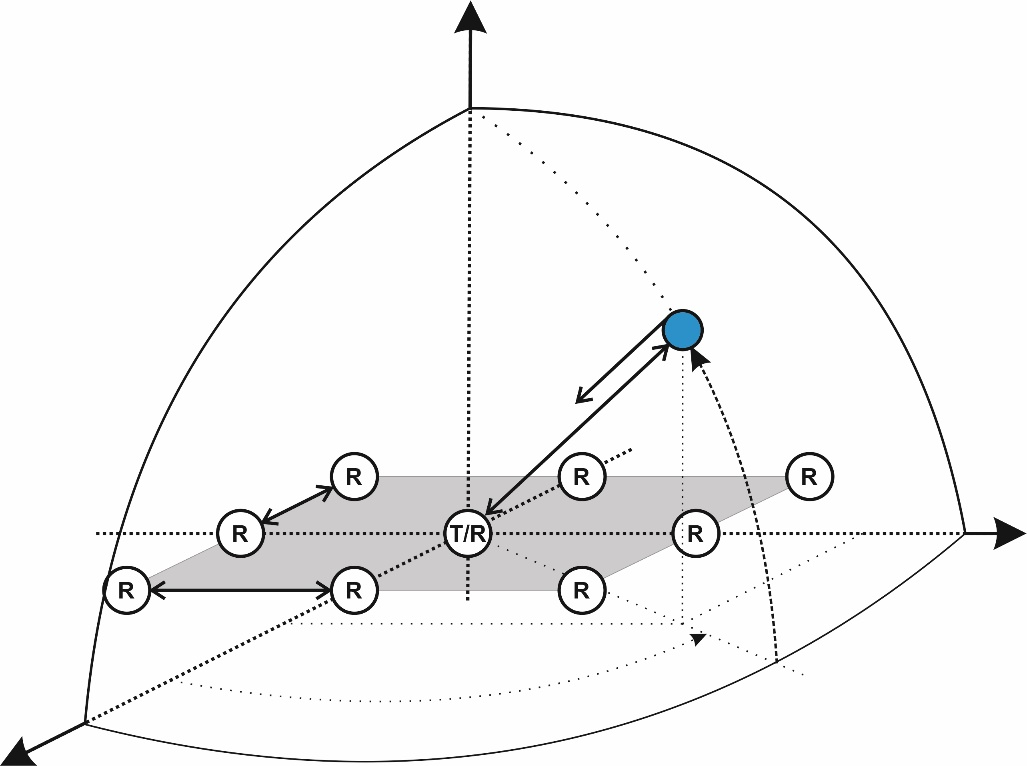
\includegraphics[width=1\linewidth]{rpresentation/atRwEi.jpg}}
	\end{minipage}
	\vfill			
	\begin{equation}
	\begin{aligned}
	\label{eq:5}
	[\ten{H}_\pai(\pars)]_{(\ti,\fri,\rxi_\te{x},\rxi_\te{y})} =\underbrace{\tgaini \cdot e^{-j2\pi \lfr \delay}}_{\gaini} \cdot 
	\underbrace{e^{-j2\pi \scs \fri \delay}}_{b_{\pai,\fri}^f} \cdot \\
	\underbrace{e^{j2\pi \frac{\color{red}\sfr\color{black} \ts\ti}{c} \vrel}}_{b_{\pai,\ti,\fri}^t} \cdot
	\underbrace{e^{-j2\pi \frac{\color{red}\sfr}{c} \delta_{\rxi_\te{x}}^{r,\te{x}}}}_{b_{\pai,\rxi_\te{x},\fri}^\te{x}}
	\underbrace{e^{-j2\pi \frac{\color{red}\sfr}{c} \delta_{\rxi_\te{y}}^{r,\te{y}}}}_{b_{\pai,\rxi_\te{y},\fri}^\te{y}}
	\end{aligned}
	\end{equation}
	\vfill
\end{frame}
\note{
	Рассматрим систему с одной передающей и массивом приёмных антенн. Формула 3 описывает параметризацию одного луча в такой системе. Как выделено в формуле, фазовые сдвиги между отдельными антеннами, равно как и набег фазы в результате Допплеровского сдвига от символа к символу зависят от частоты (выделено красным). В такой постановке параметрическое описание лучей не позволяет напрямую использовать упомянутые тензорные разложения, равно как и множество других методов оценивания, предназначенных для узкополосных систем.
	
	В связи с этим была предложена методика предварительной обработки сигналов, позволяющая уменьшить отклонения модели данных в широкополосной системы от эквивалентой узкополосной.
}

\tikzset{
	myarrow/.style={
		draw,
		fill=blue,
		single arrow,
		minimum height=3.5ex,
		single arrow head extend=1ex
	}
}
\newcommand{\arrowdown}{%
	\tikz [baseline=-1ex]{\node [myarrow,rotate=-90] {};}
}
\begin{frame}
	\frametitle{{\large Оценивание параметров широкополосных каналов связи II}}	
	\centering
	\vfill
	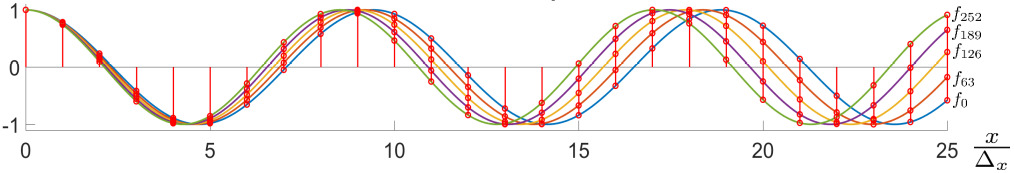
\includegraphics[width=1\linewidth]{rpresentation/wideband} \\
	\vfill
	\arrowdown
	\vfill
	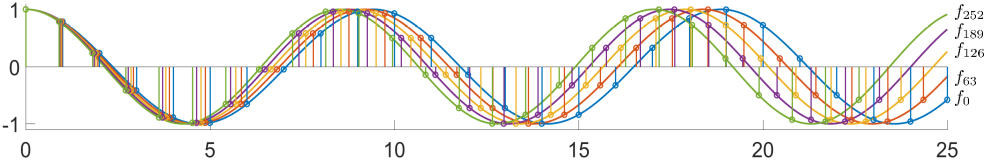
\includegraphics[width=1\linewidth]{rpresentation/iwideband}
	\vfill
	{
		\footnotesize
		\setbeamercolor{block body}{bg=brown!10}
		\setbeamercolor{block title}{bg=brown!20}
		\setbeamertemplate{blocks}[rounded][shadow]
		\begin{block}{Публикации}
			\begin{itemize}
				\item Efficient multidimensional parameter estimation for joint wideband
				radar and communication systems based on OFDM. /. — J. Zhang
				[и др.] //. — New Orleans, LA : IEEE, 2017. — С. 3096—3100.
				\item Efficient Multidimensional Wideband Parameter Estimation for
				OFDM Based Joint Radar and Communication Systems. /. —
				I. Podkurkov [и др.] // IEEE Access. — 2019. — Т. 7. —
				С. 112792—112808. 
			\end{itemize}
		\end{block}
	}
\end{frame}
\note{
	Идея заключается в следующем. Для простоты представим на рисунке изменение фазы вдоль одного измерения антенн прямоугольного массива антенн (как на рисунке на предыдущем слайде). Увеличение f\_i вызывает дополнительный набег фаз для поднесущих с высокой частотой. Однако, если подстраивать период дискретизации (расстояние между антеннами) в зависимости от частоты, можно было бы скоменсировать дополнительный набег фазы и получить данные, эквивалентные узкополосной системе. Так как физически это невозможно, простым решением является использование интерполяции для получения отсчётов с нужным периодом на каждой частоте.
}

\begin{frame}
	\frametitle{{\large Оценивание параметров широкополосных каналов связи III}}
	\begin{minipage}[с]{1.1\linewidth}
		\begin{center} 
			\textbf{Результаты компьютерного моделирования}
			\center{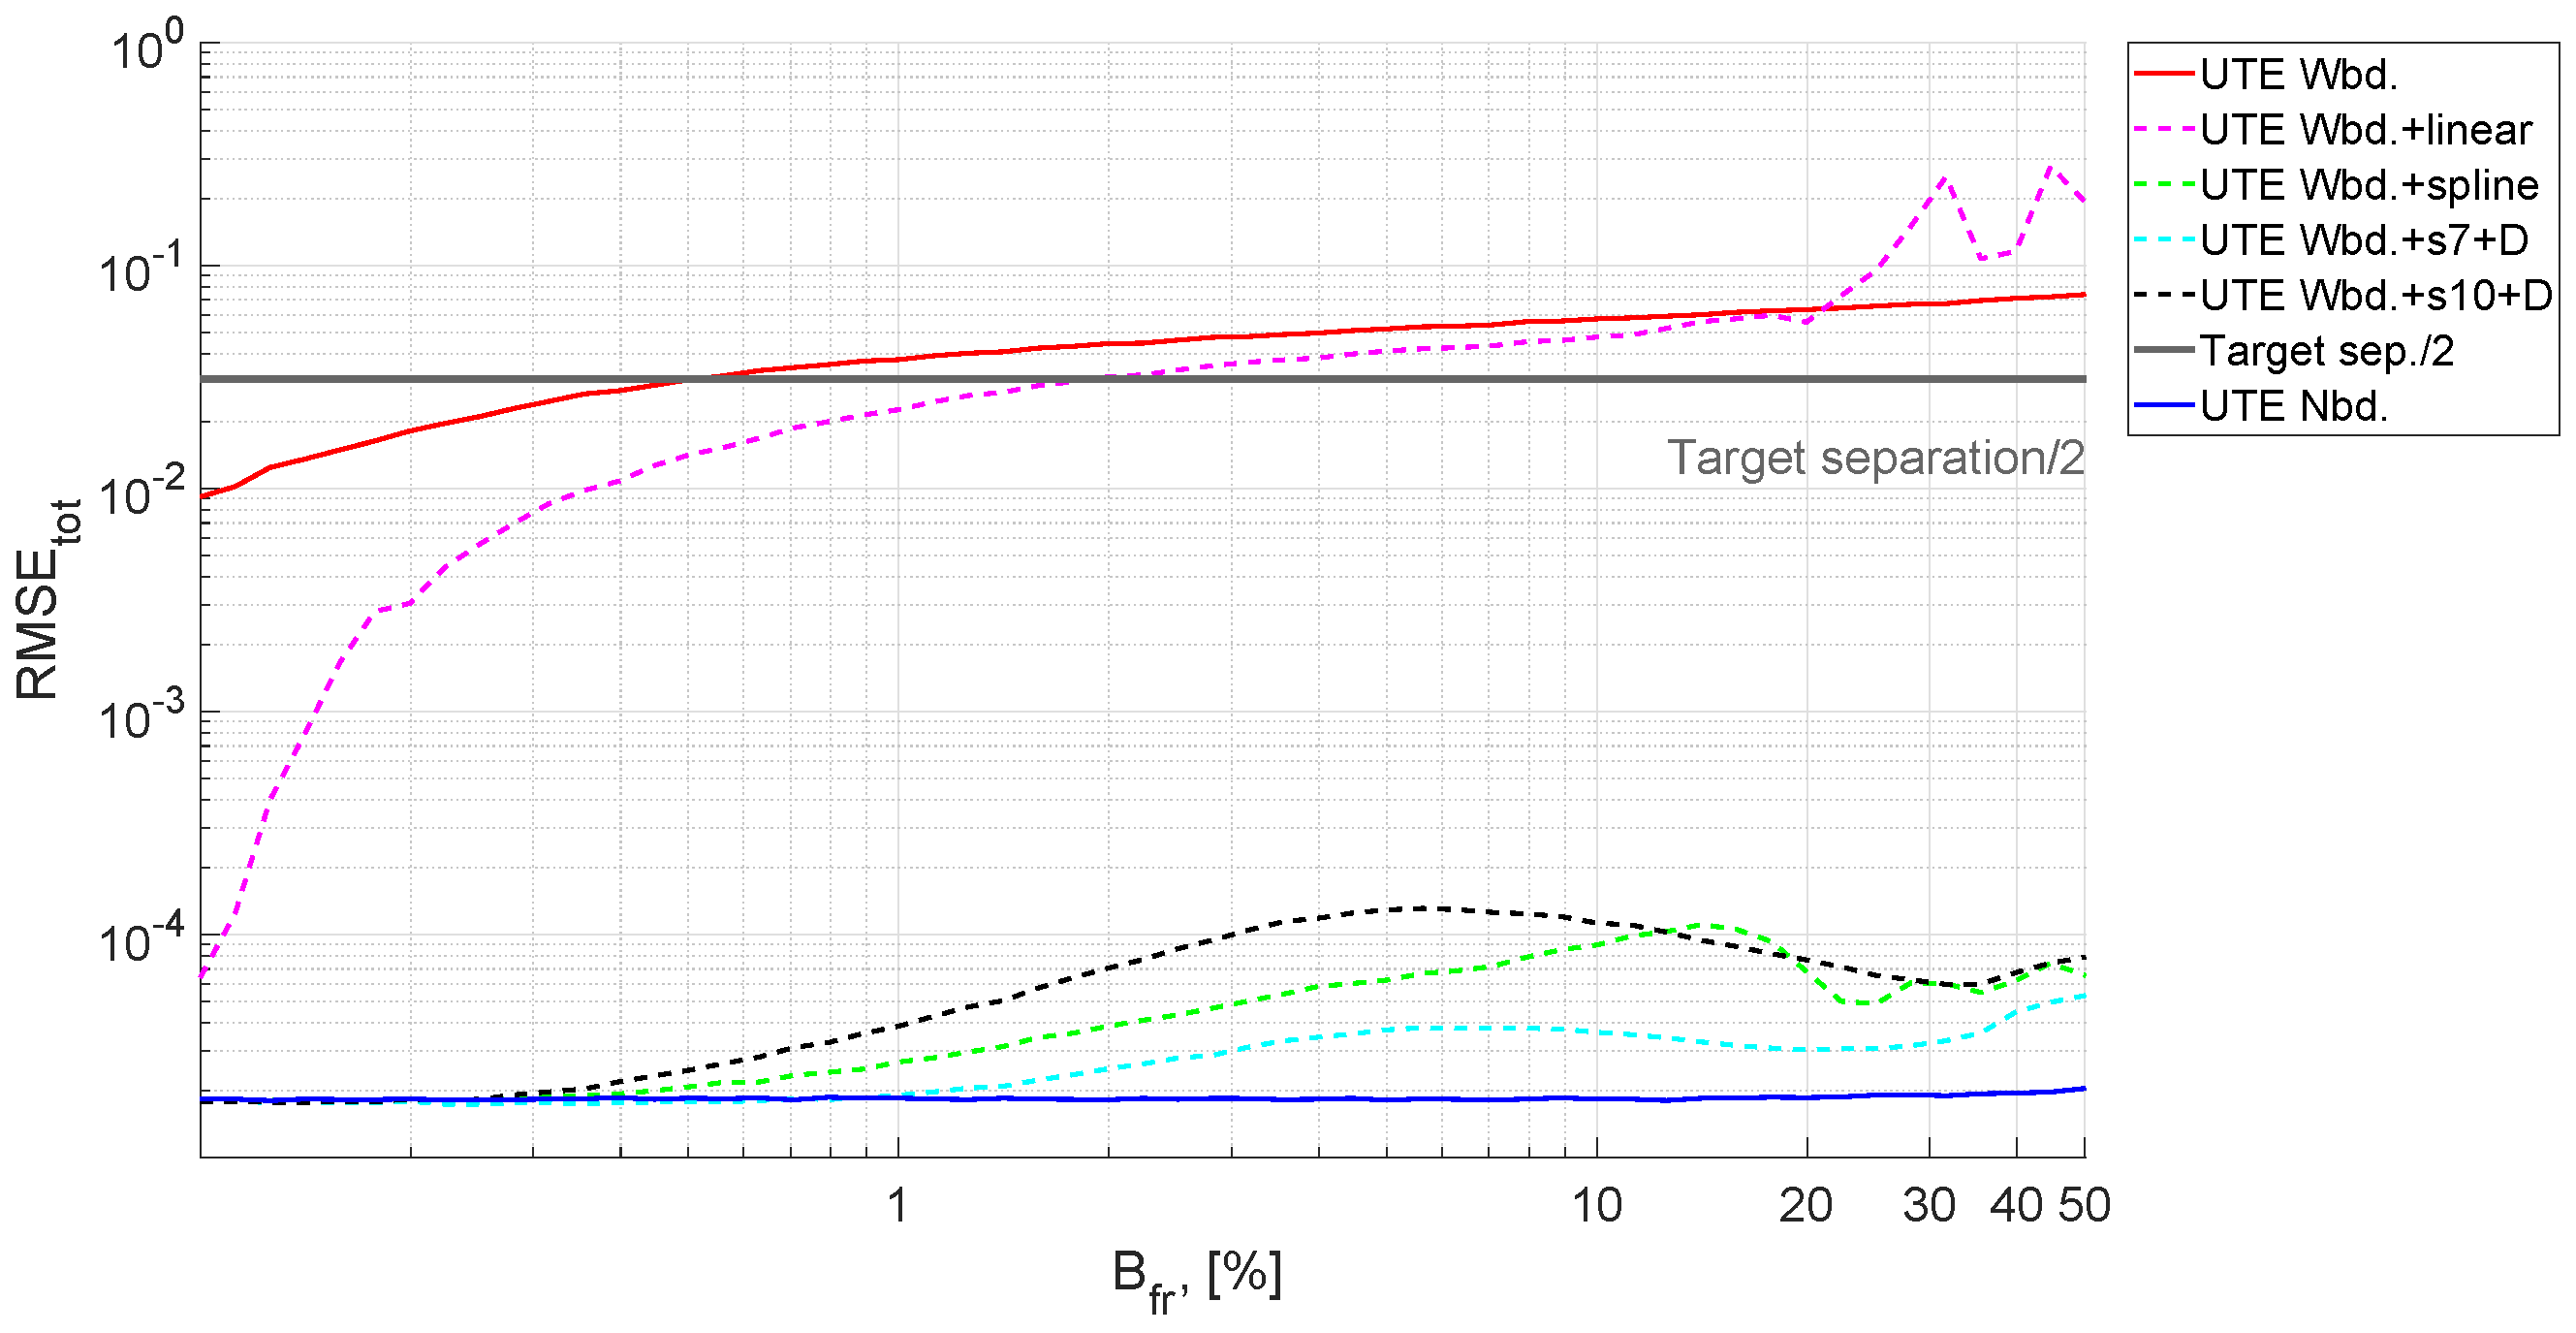
\includegraphics[width=0.8\linewidth]{FRAC_ed_final}}
		\end{center}
	\end{minipage}
	\vfill
	{
		\footnotesize		
		\setbeamercolor{block body}{bg=structure!10}
		\setbeamercolor{block title}{bg=structure!20}
		\setbeamertemplate{blocks}[rounded][shadow]
		\begin{description}
			\item [UTE] Unitary Tensor ESPRIT \cite{Haardt08}
			\item [Wbd./Nbd.] использование широкополосной/узкополосной модели данных
			\item [Linear/spline/s7/s10] интерполяция с помощью сплайнов 1/3/7/10 порядка, соответственно
		\end{description}
	}
\end{frame}
\note{
	Результаты компьютерного моделирования показывают, что применение предварительной обработки с помощью интерполяции данных позволяет существенно увеличить эффективность оценивания в широкополосной системе, в то же время имея возвожность использовать узкополосный алгоритмы оценивания.
}


\section{Оценивание параметров каналов связи в ближнем поле}

\begin{frame}
	\frametitle{{\large Оценивание параметров каналов связи в ближнем поле I}}
	
	\begin{minipage}[t]{0.47\linewidth}
		{
			\setbeamercolor{block body}{bg=structure!10}
			\setbeamercolor{block title}{bg=structure!20}
			\setbeamertemplate{blocks}[rounded][shadow]
			\begin{block}{}
				\begin{itemize}
					\item Рассматривается MIMO Radar система \cite{Singh2017a} \cite{Podkurkov2018}
					\item Используется сферическая модель фронта волны
				\end{itemize}		
			\end{block}
		}
	\end{minipage}
	\hfill
	\begin{minipage}[t]{0.47\linewidth}
		\begin{center} \textbf{Сферический фронт волны}
		\end{center}
		\center{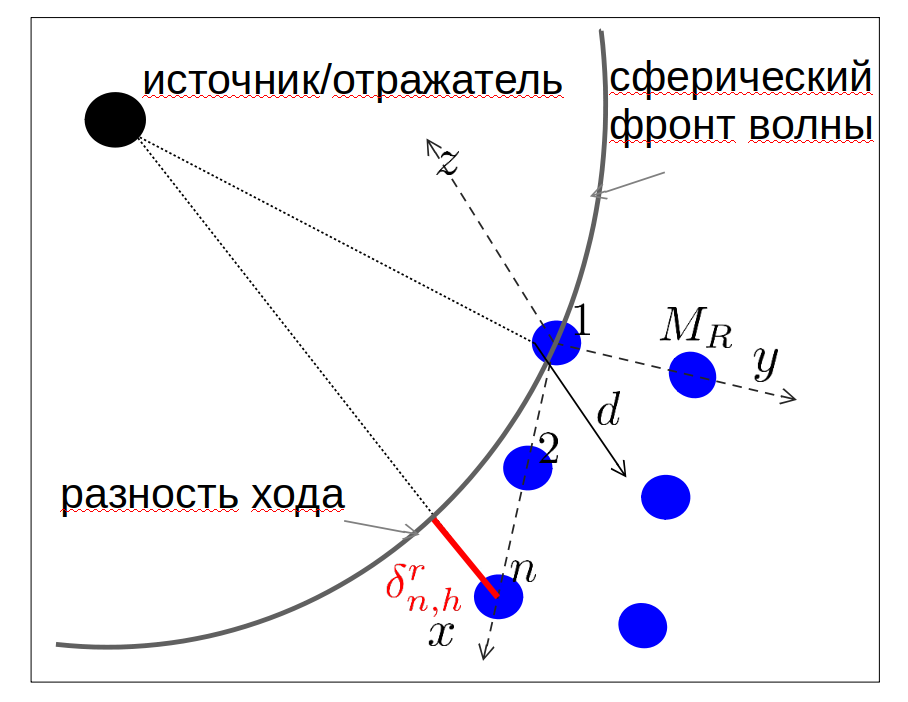
\includegraphics[width=1\linewidth]{rpresentation/nearfield}}
	\end{minipage}
	\vfill			
	\begin{equation}
	\label{eq:6}
	\delta_{\rxi,\pai} = \sqrt{ (x_\pai-x_\rxi)^2 + (y_\pai-y_\rxi)^2 + (z_\pai-z_\rxi)^2} -\rho_\pai\text{\ \ }\forall \rxi,\pai	
	\end{equation}
	\vfill	
	\begin{description}
		\item[$x_\rxi$, $y_\rxi$, $z_\rxi$] Декартовы координаты $\rxi$-й приёмной антенны
		\item[$x_\pai$, $y_\pai$, $z_\pai$] Декартовы координаты $\pai$-го источника/отражателя антенны
		\item[$\rho_\pai$] расстояние до $\pai$-го источника/отражателя антенны
	\end{description}
\end{frame}
\note{
	Тензорные разложения открывают новые возможности для построения алгоритмов оценивания каналов связи. В частности, использование Канонического тензорного разложения в системе с отражателями/источниками в ближнем геометрическом поле позволило разработать новый алгоритм определения углов прихода сигналов и расстояния с использованием сферической модели фронта волны, для которой разности хода фронта между антеннами имеют нелинейную зависимость от положения источника/отражателя.
}

\begin{frame}
	\frametitle{{\large Оценивание параметров каналов связи в ближнем поле II}}
	
	\begin{minipage}[t]{0.3\linewidth}
		{
			\small
			\setbeamercolor{block body}{bg=structure!10}
			\setbeamercolor{block title}{bg=structure!20}
			\setbeamertemplate{blocks}[rounded][shadow]
			\begin{block}{}
				Разработан алгоритм локализации источников \cite{Podkurkov2018}, позволяющий получать несмещённые оценки азимута, угла места и расстояния до источника/отражателя с использованием произвольной геометрии приёмного массива антенн		
			\end{block}
		}
	\end{minipage}
	\hfill
	\begin{minipage}[t]{0.64\linewidth}
		\begin{center}
			\textbf{Результаты компьютерного моделирования}
		\end{center}
		\center{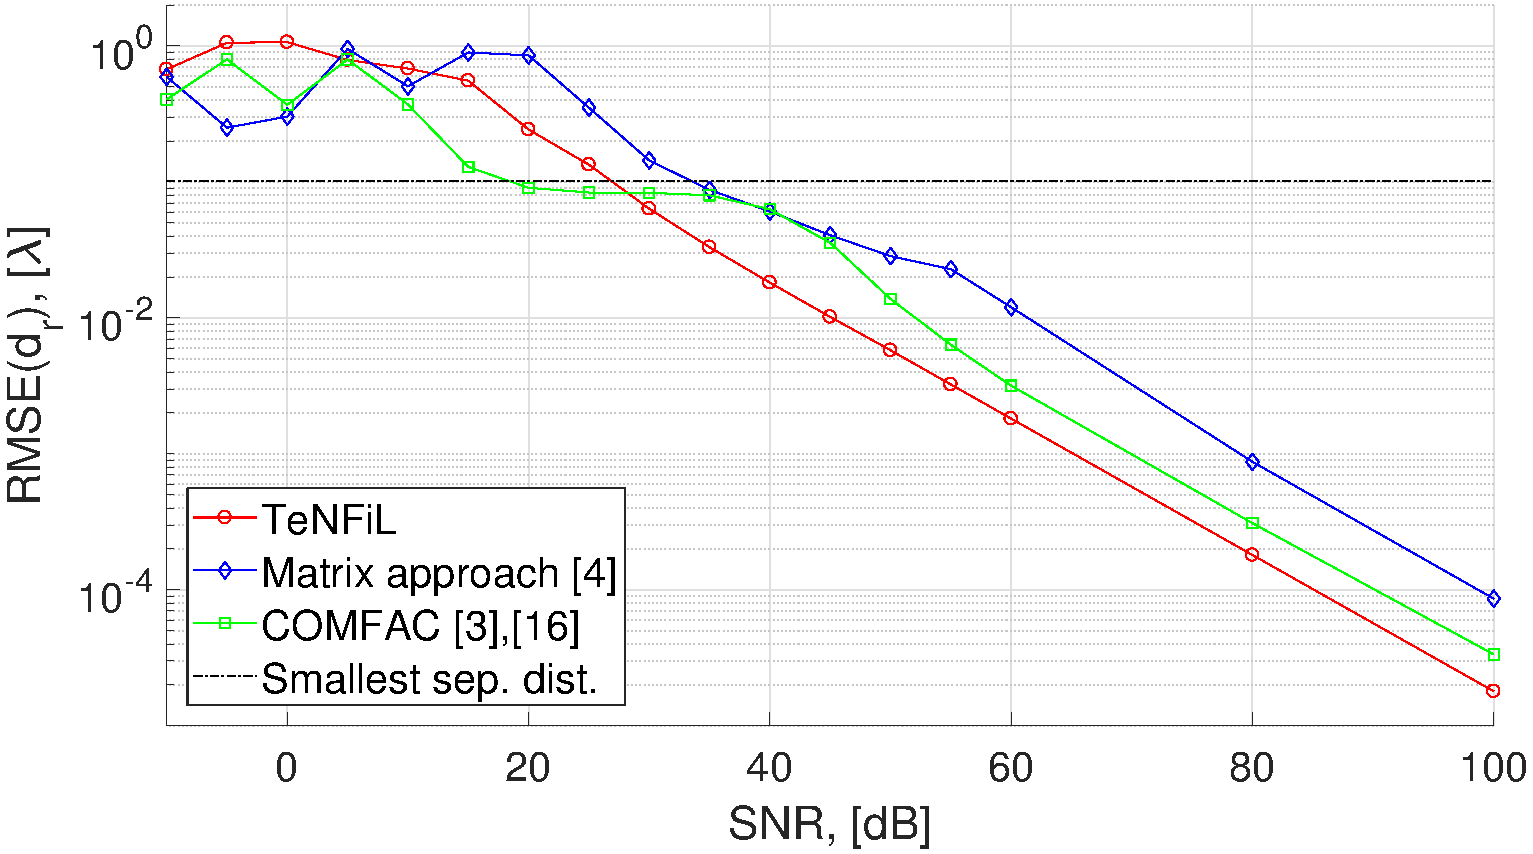
\includegraphics[width=1\linewidth]{mse_dt_onenan}}
		\vfill
		\begin{description}
			\item[TeNFiL] - разработанный метод оценивания
		\end{description}
	\end{minipage}
	\vfill
	{
		\footnotesize
		\setbeamercolor{block body}{bg=brown!10}
		\setbeamercolor{block title}{bg=brown!20}
		\setbeamertemplate{blocks}[rounded][shadow]
		\begin{block}{Публикации}
			\begin{itemize}
				\item Tensor-Based Near-Field Localization in Bistatic MIMO Radar
				Systems. /. — I. Podkurkov [и др.] //. — Bochum, Germany :
				VDE, 2018. — С. 1—8.
			\end{itemize}
		\end{block}
	}
\end{frame}
\note{
	Каноническое разложение позволило получить точные фазовые сигнатуры источников на приёмном массиве антенн, дающие возможность получить несмещённые оценки положения (углов прихода и расстояния). На графике изображено сравнение с аналогичными алгоритмами, TeNFiL - предложенный метод.
}

\section{Анализ потенциальных характеристик оценивания параметров каналов связи.}

\begin{frame}
	\frametitle{Анализ потенциальных характеристик оценивания параметров каналов связи I}
	{
		\setbeamercolor{block body}{bg=structure!10}
		\setbeamercolor{block title}{bg=structure!20}
		\setbeamertemplate{blocks}[rounded][shadow]
		\begin{block}{}
			\begin{itemize}
				\item Аддитивная помеха имеет распределение в виде произвольной смеси Гауссовских распределений
				\item Анализ проводится с помощью вычисления границы Крамера-Рао
			\end{itemize}		
		\end{block}
	}
	{
	\setbeamercolor{block body}{bg=structure!10}
	\setbeamercolor{block title}{bg=structure!20}
	\setbeamertemplate{blocks}[rounded][shadow]
	\begin{block}{Метод вычисления границы Крамера-Рао}
		\begin{itemize}
			\item Аппроксимация промежуточной ("шумовой") матрицы Фишера с помощью метода Монте-Карло
		\end{itemize}	
	\end{block}
	}
	{
		\footnotesize
		\setbeamercolor{block body}{bg=brown!10}
		\setbeamercolor{block title}{bg=brown!20}
		\setbeamertemplate{blocks}[rounded][shadow]
		\begin{block}{Публикации}
			\begin{itemize}
				\item Подкурков, И. А. — Потенциальные характеристики оценивания
				направлений прихода сигналов в условиях негауссовских
				помех. /. — И. А. Подкурков, А. Ф. Надеев // Вестник
				Марийского государственного технического университета.
				Серия: Радиотехнические и инфокоммуникационные
				системы. — 2019. — Т. 1, No 4. — С. 16—26.
			\end{itemize}
		\end{block}
	}		
\end{frame}
\note{
	Анализ потенциальных характеристик осуществлялся с помощью численной аппроксимации границы Крамера-Рао, полученной с помощью метода Монте-Карло. При этом сначала аппроксимируется промежуточная матрица Фишера задачи, в которой неизвестными параметрами считаются отсчёты шума/помехи. Далее, вычисление матрицы Фишера относительно неизвестных параметров осуществляеются с помощью преобразования смены переменных и инверсии полученной матрицы.
	
	Стоит отметить, что вычисление границы Крамера-Рао для произвольного распределения помехи является крайне сложной задачей, в частности для смесевых распределений и в литературе встречается лишь для частных случаев.
}

\begin{frame}
	\frametitle{Анализ потенциальных характеристик оценивания параметров каналов связи II}
	\begin{minipage}[t]{0.47\linewidth}
		\begin{center}
			\textbf{Результаты компьютерного моделирования}
		\end{center}
		\center{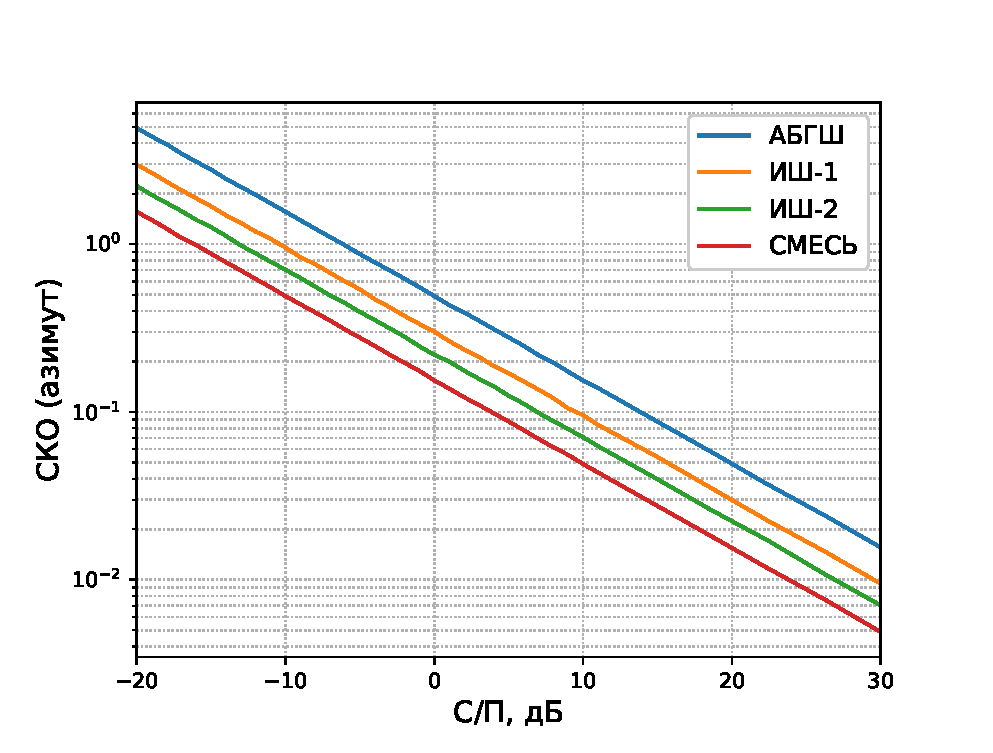
\includegraphics[width=1.3\linewidth]{Fig_2}}
	\end{minipage}
	\hfill
	\begin{minipage}[t]{0.47\linewidth}
		{
			\scriptsize
			\begin{description}
				\item [АБГШ] Аддитивный Белый Гауссовский шум
				\item [ИШ-1] аддитивная помеха задана циклично-симметричной смесью двух компонент с различными дисперсиями ("импульсный шум")
				\item [ИШ-2] аддитивная помеха задана смесью двух компонент с различными дисперсиями и корреляцией между квадратурными компонентами шума
				\item [СМЕСЬ] произвольная смесь компонент с ненулевыми средними и одинаковыми кофариацонными матрицами
			\end{description}	
		}
	\end{minipage}

\end{frame}
\note{
	Результаты моделирования показывают, что помеха заданная более сложным распределением потенциально позволяет обеспечивать более высокое качество оценивания искомых параметров.
}

\begin{comment}
\section{Списки}
\begin{frame}[plain, noframenumbering]
    \begin{center}
        \Huge
        Списки
    \end{center}
\end{frame}

\subsection{Нумерованные}

\begin{frame}
    \frametitle{Нумерованные списки}
    \begin{enumerate}
        \item один
        \item два
        \item три
    \end{enumerate}
\end{frame}
\note{
    Этот текст будет виден только если его отображение включено в файле \textbf{Presentation/setup}.
    Для раздельного вывода презентации и заметок на разные экраны (как в impress или powerpoint) можно использовать программу \textit{pdf-presenter-console}.
}

\subsection{Не нумерованные}


\begin{frame}
    \frametitle{Перечисления}
    \begin{itemize}
        \item Проблема 1
        \item Проблема 2
        \item Проблема 3
    \end{itemize}
\end{frame}
\note[itemize]{
    \item Тезис 1
    \item Тезис 2
    \item Тезис 3
}

\subsection{Комбинированные}

\begin{frame}
    \frametitle{Комбинация списков}
    \begin{enumerate}
        \item \textbf{Задача 1}
              \begin{itemize}
                  \item Подзадача 1-1
                  \item Подзадача 1-2
              \end{itemize}
        \item \textbf{Задача 2}
              \begin{itemize}
                  \item Подзадача 2-1
                  \item Подзадача 2-2
                  \item Подзадача 2-3
              \end{itemize}
        \item \textbf{Задача 3}
              \begin{itemize}
                  \item Подзадача 3-1
                  \item Подзадача 3-2
                  \item Подзадача 3-3
              \end{itemize}
    \end{enumerate}
\end{frame}
\note[itemize]{
    \item Задача 1
    \item Задача 2
    \item Задача 3
}

\begin{frame}[allowframebreaks]
    \frametitle{Разделение слайда}
    Поясняющий текст
    \begin{itemize}
        \item Один
        \item Два
        \item Три
    \end{itemize}
    \framebreak
    Продолжение предыдущего слайда
\end{frame}

\section{Графика}
\begin{frame}[plain, noframenumbering]
    \begin{center}
        \Huge
        Графика
    \end{center}
\end{frame}


\begin{frame}
    \frametitle{Одиночное изображение}
    \centering
    \includegraphics[width=0.8\linewidth]{latex} % окружение figure не требуется
\end{frame}

\begin{frame}
    \frametitle{Векторная графика}
    \begin{figure}
	    \centering
	    \ifdefmacro{\tikzsetnextfilename}{\tikzsetnextfilename{tikz_presentation}}{}% присваиваемое предкомпилированному pdf имя файла (не обязательно)
	    \input{Presentation/images/tikz_plot.tikz}
    \end{figure}
\end{frame}

\subsection{Расположение}

\begin{frame}
    \frametitle{Изображения по-вертикали}
    \centering
    \vfill
    \includegraphics[width=0.8\linewidth,height=0.1\textheight]{latex} \\
    \TeX
    \vfill
    \includegraphics[width=0.8\linewidth,height=0.2\textheight]{latex} \\
    \LaTeX
    \vfill
    \includegraphics[scale=0.2]{latex} \\
    \vfill
\end{frame}


\begin{frame}
    \frametitle{Изображения по-горизонтали}
    \begin{minipage}[t]{0.47\linewidth}
        \textbf{Составная \\ подпись 1}
        \center{\includegraphics[width=1\linewidth]{knuth1}}
    \end{minipage}
    \hfill
    \begin{minipage}[t]{0.47\linewidth}
        \textbf{Составная \\ подпись 2}
        \center{\includegraphics[width=1\linewidth]{knuth2}}
    \end{minipage}
\end{frame}

\subsection{Линии}

\begin{frame}
    \frametitle{Разделяющие линии}
    \begin{minipage}[c]{0.47\linewidth}
        \center{\includegraphics[width=1\linewidth]{latex}}
        \bigskip
        \hrule{}
        \bigskip
        \textbf{Составная \\ подпись 1}
    \end{minipage}
    \hfill
    \vrule{}
    \hfill
    \begin{minipage}[c]{0.47\linewidth}
        \flushright
        \textbf{Составная \\ подпись 2}
        \center{\includegraphics[width=1\linewidth]{knuth2}}
    \end{minipage}
\end{frame}

\section{Остальное}
\begin{frame}[plain, noframenumbering]
    \begin{center}
        \Huge
        Остальное
    \end{center}
\end{frame}

\subsection{Формулы}

\begin{frame}
    \frametitle{Формулы}
    \[
    \left\{
    \begin{array}{rl}
        \dot x = & \sigma (y-x)  \\
        \dot y = & x (r - z) - y \\
        \dot z = & xy - bz
    \end{array}
    \right.
    \]
\end{frame}

\begin{frame}
    \frametitle{amsmath}
    \centering
    \begin{minipage}[t]{0.5\linewidth}
        \begin{multline*}
            y = 1 x^1 + 2 x^2 + 3 x^3 + \\ + 4 x^4 + 5 x^5 + \dots
        \end{multline*}
    \end{minipage}
\end{frame}

\begin{frame}[allowframebreaks]
    \frametitle{Уравнения Максвелла}
    \centering{
        \small
        \def\arraystretch{1.8}%
        \begin{tabular}{ll}
            \toprule
            Интегральная форма                                                                                                                                          & Дифференциальная форма                                                        \\ \midrule
            \(Q_e(t) = \displaystyle\oiint_S \vec D(t) \cdot d\vec{s} = \displaystyle\iiint_V \rho_v(t) dv\)                                                              & \(\nabla \cdot \vec D(t) = \rho_v(t)\)                                          \\
            \(\displaystyle\oiint_S \vec B(t) \cdot d\vec{s} = 0\)                                                                                                        & \(\nabla \cdot \vec B(t) = 0\)                                                  \\
            \(V_{emf}(t) = \displaystyle\oint_L \vec E(t) \cdot d\vec{l}\) = \(- \displaystyle\iint_S \left[\frac{\partial\vec{B}(t)}{\partial t}\right] \cdot d\vec{s}\)   & \(\nabla \times \vec E(t) = - \frac{\partial\vec{B}(t)}{\partial t}\)           \\
            \(I(t) = \displaystyle\oint_L \vec H(t) \cdot d\vec{l} = \displaystyle\iint_S \left[\vec J(t) + \frac{\partial\vec{D}(t)}{\partial t}\right] \cdot d\vec{s}\) & \(\nabla \times \vec H(t) = \vec J(t) + \frac{\partial\vec{D}(t)}{\partial t}\) \\ \midrule
            \(\displaystyle\oiint_S \vec J \cdot d\vec{s} = -\frac{\partial Q_e}{\partial t}\)                                                                            & \(\nabla \cdot \vec J = - \frac{\partial \rho_v}{\partial t}\)                  \\
            \bottomrule
            \multicolumn{2}{c}{\(\vec D(t) = \left[\varepsilon(t)\right] * \vec E(t)\)}                                                                                                                                                                   \\
            \multicolumn{2}{c}{\(\vec B(t) = \left[\mu(t)\right] * \vec H(t)\)}                                                                                                                                                                           \\
        \end{tabular}
    }
    \framebreak

    \hspace{0.05\linewidth}
    \centering{
        \small
        \def\arraystretch{1.8}%
        \begin{tabular}{ll}
            \toprule
            Интегральная форма                                                                                                            & Дифференциальная форма                             \\ \midrule
            \(Q_e = \displaystyle\oiint_S \vec D \cdot d\vec{s} = \displaystyle\iiint_V \rho_v dv\)                                         & \(\nabla \cdot \vec D = \rho_v\)                     \\
            \(\displaystyle\oiint_S \vec B \cdot d\vec{s} = 0\)                                                                             & \(\nabla \cdot \vec B = 0\)                          \\
            \(V_{emf} = \displaystyle\oint_L \vec E \cdot d\vec{l}\) = \(- \displaystyle\iint_S \left[j \omega \vec B\right] \cdot d\vec{s}\) & \(\nabla \times \vec E = - j \omega \vec B\)         \\
            \(I = \displaystyle\oint_L \vec H \cdot d\vec{l} = \displaystyle\iint_S \left[\vec J + j \omega \vec D\right] \cdot d\vec{s}\)  & \(\nabla \times \vec H = \vec J + j \omega \vec{D}\) \\ \midrule
            \(\displaystyle\oiint_S \vec J \cdot d\vec{s} = - j \omega Q_e\)                                                                & \(\nabla \cdot \vec J = - j \omega \rho_v\)          \\
            \bottomrule
            \multicolumn{2}{c}{\(\vec D(t) = \left[\varepsilon\right] \vec E(t)\)}                                                                                                               \\
            \multicolumn{2}{c}{\(\vec B(t) = \left[\mu\right] \vec H(t)\)}                                                                                                                       \\
        \end{tabular}
    }
\end{frame}

\subsection{Таблицы}

\begin{frame}
    \frametitle{Таблица}
    \centering
    \begin{tabular}{|l|l|}
        \hline
        \textbf{Заголовок 1} & \textbf{Заголовок 2} \\
        \hline
        Сумма                & \(b+a\)                \\
        \hline
        Разность             & \(a-b\)                \\
        \hline
        Произведение         & \(a*b\)                \\
        \hline
    \end{tabular}
\end{frame}

\begin{frame}
    \frametitle{Другая таблица}
    \centering
    \begin{tabular}{lc}
        \toprule
        \multicolumn{1}{c}{\textbf{Заголовок 1}} & \textbf{Заголовок 2} \\ \midrule
        Сумма                                    & \(b+a\)                \\
        Разность                                 & \(a-b\)                \\
        Произведение                             & \(a*b\)                \\
        \bottomrule
    \end{tabular}
\end{frame}


\subsection{Разное}

\begin{frame}
    \frametitle{Большой многоуровневый список}
    \begin{itemize}
        \item \textbf{Пункт 1}
              \begin{itemize}
                  \itemi Подпункт 1-1
                  \itemi Подпункт 1-2
              \end{itemize}
        \item \textbf{Пункт 2}
              \begin{itemize}
                  \itemi Подпункт 2-1
              \end{itemize}
        \item \textbf{Пункт 3}
              \begin{itemize}
                  \itemi Подпункт 3-1
                  \itemi Подпункт 3-2
              \end{itemize}
        \item \textbf{Пункт 4}
              \begin{itemize}
                  \itemi Подпункт 4-1
              \end{itemize}
        \item \textbf{Пункт 5}
              \begin{itemize}
                  \itemi Подпункт 5-1
                  \itemi Подпункт 5-2
                  \itemi Подпункт 5-3
              \end{itemize}
    \end{itemize}
\end{frame}

\begin{frame}
    \frametitle{Четыре изображения}
    \centering
    \includegraphics[width=0.35\linewidth,angle=35]{latex}
    \includegraphics[width=0.35\linewidth,angle=135]{latex}\\
    \includegraphics[width=0.35\linewidth,angle=15]{latex}
    \includegraphics[width=0.35\linewidth,angle=-15]{latex}
\end{frame}
\end{comment}       % Настройки заглавной странице
\begin{frame}
	\frametitle{Заключение}
	\begin{itemize}
		\item Предложенный метод предварительной обработки многомерных сигналов в широкополосных системах позволяет применять алгоритмы оценивания параметров каналов связи, разработанные для узкополосных систем.
		\item Разработан новый алгоритм оценивания параметров канала связи с отражателями в ближнем геометрическом поле с использованием сферической модели фронта волны.
		\item Исследована граница Крамера-Рао для задач оценки параметров каналов связи с негауссовым распределением аддитивной помехи, заданным смесью нормальных распределений с ненулевыми средними значениями компонент.
	\end{itemize}
\end{frame}
\note{
	Проговариваются основные заключения
}

\begin{comment}
\begin{frame}
    \frametitle{Научная новизна}
    \begin{itemize}
        \item Впервые реализован \dots
        \item Разработана программа \dots
        \item Впервые проведён анализ \dots
        \item Предложена схема \dots
    \end{itemize}
\end{frame}
\note{
    Проговаривается вслух научная новизна
}

\begin{frame}
    \frametitle{Научная и практическая значимость}
    \begin{itemize}
        \item Получены выражения для \dots.
        \item Определены условия \dots.
        \item Разработаны устройства \dots.
    \end{itemize}
\end{frame}
\note{
    Проговариваются вслух научная и практическая значимость
}

\begin{frame}
    \frametitle{Свидетельство о регистрации программы}
    \begin{figure}[h]
        \centering
        \includegraphics[height=0.7\textheight]{registration}
    \end{figure}
\end{frame}
\note{
    Получено свидетельство о регистрации разработанной программы \textsc{Hello~world™}.
}

\begin{frame}
    \frametitle{Акт о внедрении}
    \begin{figure}[h]
        \centering
        \fbox{
            \begin{minipage}[t]{0.4\linewidth}
                \includegraphics[width=\linewidth]{implementation}
            \end{minipage}
        }
    \end{figure}
\end{frame}
\note{
    Получен акт о внедрении.
}
\end{comment}

\begin{frame}[t,allowframebreaks] % публикации на нескольких страницах
	\frametitle{Список литературы}	
	
	%% authorvak
	\nocite{vakbib1}%
	\nocite{vakbib2}%
	%
	%% authorwos
	%
	%% authorscopus
	\nocite{Zhang2017}%
	\nocite{Podkurkov2017}%
	\nocite{Podkurkov2019}
	%
	%% authorconf
	\nocite{Podkurkov2018}%
	%% authorother
	\nocite{otherbib1}%
	
	\ifnumequal{\value{bibliosel}}{0}{
		\insertbiblioexternal%
	}{	
		\printbibliography%
	}
\end{frame}
\note{
	Список литературы цитируемой в тексте презентации
}

\begin{comment}
\begin{frame}
    \frametitle{Участие в конференциях}
    \begin{itemize}
        \item Научная сессия МГУ, Москва 2013--2015;
        \item \rom{24} Russian Conference (RuC 2014), Obninsk, Russia, 2014
        \item \rom{7} International Conference (IAC 16), Busan, Korea,
              2016;
        \item \rom{28} Other Conference (AC 16), East Lansing, MI USA, 2016;
        \item \dots
    \end{itemize}
\end{frame}
\note{
    Работа была представлена на ряде конференций.
}
\end{comment}

\begin{frame}[plain, noframenumbering] % последний слайд без оформления
    \begin{center}
        \Huge
        Спасибо за внимание!
    \end{center}
\end{frame}
    % Последние слайды презентации
\appendix
\begin{comment}
\begin{frame}
    \frametitle{Ответы на замечания ведущей организации НИИ~<<Рога~и~копыта>>}
    \begin{itemize}
        \item Замечание -- ответ
        \item Замечание -- ответ
        \item Замечание -- ответ
        \item Замечание -- ответ
        \item Замечание -- ответ
    \end{itemize}
\end{frame}

\begin{frame}
    \frametitle{Ответы на замечания оф. оппонента Иванова\,И.\,И}
    \begin{itemize}
        \item Замечание -- ответ
        \item Замечание -- ответ
        \item Замечание -- ответ
        \item Замечание -- ответ
        \item Замечание -- ответ
    \end{itemize}
\end{frame}

\begin{frame}
    \frametitle{Ответы на замечания Петрова\,П.\,П}
    \begin{itemize}
        \item Замечание -- ответ
        \item Замечание -- ответ
        \item Замечание -- ответ
        \item Замечание -- ответ
        \item Замечание -- ответ
    \end{itemize}
\end{frame}
\end{comment}
      % Запасные слайды презентации
\end{document}
